% This is a simple LaTex sample document that gives a submission format
%   for IEEE PAMI-TC conference submissions.  Use at your own risk.

% Make two column format for LaTex 2e.
\documentclass[10pt,twocolumn]{article}
\usepackage{times}
\usepackage{graphicx}

% Use following instead for LaTex 2.09 (may need some other mods as well).
% \documentstyle[times,twocolumn]{article}

% Set dimensions of columns, gap between columns, and paragraph indent 
\setlength{\textheight}{8.875in}
\setlength{\textwidth}{6.875in}
\setlength{\columnsep}{0.3125in}
\setlength{\topmargin}{0in}
\setlength{\headheight}{0in}
\setlength{\headsep}{0in}
\setlength{\parindent}{1pc}
\setlength{\oddsidemargin}{-.1875in}  % Centers text.
\setlength{\evensidemargin}{-.1875in}

% Add the period after section numbers.  Adjust spacing.
\newcommand{\Section}[1]{\vspace{-8pt}\section{\hskip -1em.~~#1}\vspace{-3pt}} 
\newcommand{\SubSection}[1]{\vspace{-3pt}\subsection{\hskip -1em.~~#1}
     	\vspace{-3pt}}


\begin{document}

% Don't want date printed
\date{}

% Make title bold and 14 pt font (Latex default is non-bold, 16pt) 
\title{\Large\bf Classification of neurons of Drosophila using varying methods and feature engineering }

% For single author (just remove % characters)
%\author{I. M. Anonymous \\
%  My Department \\
%  My Institute \\
%  My City, STATE, zip}

% For two authors (default example)
\author{\begin{tabular}[t]{c@{\extracolsep{8em}}c} 
I. M. Anonymous  & M. Y. Coauthor \\
 \\
        My Department & Coauthor Department \\
        My Institute & Coauthor Institute \\
        City, STATE~~zipcode & City, STATE~~zipcode
\end{tabular}}

\maketitle


\section*{\centering Abstract}

{\em
Classification of data through the use of automated systems is wildly used in the scientific community, as it is a faster and more efficient way of arranging datasets than doing so manually. There are many classification methods, the efficiency of each depending on the dataset it works on and how the method is used.  In addition, the idea of feature selection was also visited during this project. The goal of this project was to test classification and feature selection methods. To reach this goal a main focus was observing the accuracies of these methods as their parameters were changed.
%end italics mode
}

\Section{Introduction}

Here is my introduction text.  The section heading is in a large
bold font and all sections and subsections are numbered.

Type your main text in 10-point Times, single-spaced at 12pt. Do not
use double-spacing. All paragraphs should be indented 1 pica
(approximately 1/6- or 0.17-inch or 0.422 cm). Be sure your text is
fully justified---that is, flush left and flush right. Please do not
place any additional blank lines between paragraphs.

\SubSection{Previous Work}

There are various bibliographic and citation schemes available in
LaTex, but we choose to use the simplest one in this example.
Throughout I may cite references of the form \cite{key:foo} or
\cite{foo:baz}, and LaTeX will keep track of numbering.  The numbers
are based on the order you place them in the bibliography, not the
order they appear in the text.  They should (I believe) be in
alphabetical order.  LaTex will put square brackets about the number
within the text of your paper.  For those of you new to LaTex, you may
have to run the latex process twice to allow all references to be
resolved. You will get a warning about a missing .aux file.  Just
rerun latex and it will be ok (fig. \ref{fig:chi2}).

\Section{Methods}
With the goal being to test certain methods and achieve the highest accuracy possible, we adjusted the code to make it more efficient. After receiving the data, we stored the known class of each neuron in a separate variable. This allowed us to, following the automatic classification, compare the class that the classifier assigned each neuron to versus the actual one. The classifiers we tested were K-Nearest Neighbors, Decision Tree, Random Forest, Logistic Regression, Support Vector Machine and Ensemble.






\Section{Results}

The format of the output remained the same for all six, printing out the accuracy of each iteration, the total accuracy, the name of the classifier as well as all its parameters, and finally a confusion matrix as a visual for the results. 

\begin{center}
	\begin{tabular}{||c c c c||} 
		\hline
		Method Name & Total Accuracy \\ [0.5ex] 
		\hline\hline
		Random Forest & 0.6803 \\ 
		\hline
		K-Nearest Neighbors & 0.6509 \\
		\hline
		Ensemble & 0.6741 \\
		\hline
		Decision Tree & 0.5799 \\
		\hline
		Logistic Regression & 0.5355 \\ 
		\hline
		Support Vector Machine & 0.5341 \\ [1ex] 
		\hline
	\end{tabular}
\end{center}

\begin{figure}[htbp] 
	\begin{minipage}{0.5\linewidth} 
		\centering 
		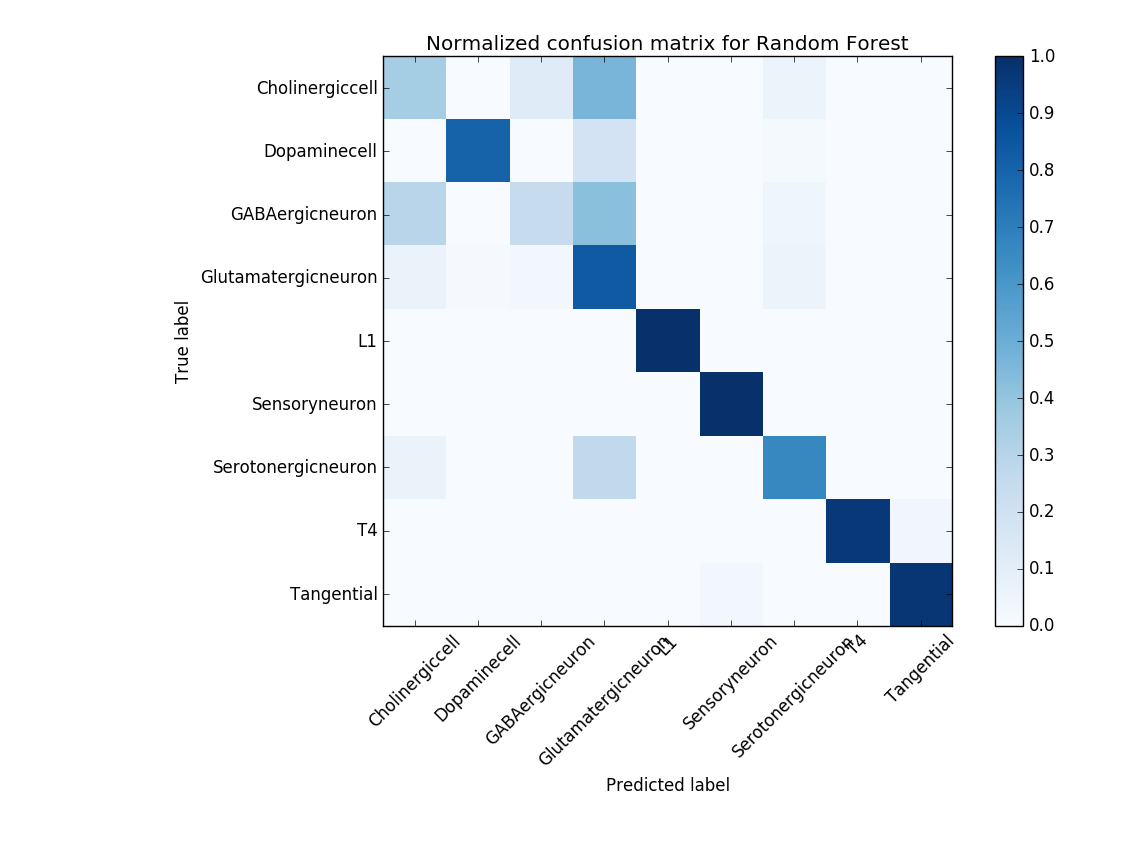
\includegraphics[width=\textwidth]{img/RFmatrix.png} 
		\caption{A Circle} 
		\label{fig:circle} 
	\end{minipage}% 
	\begin{minipage}{0.5\linewidth} 
		\centering 
		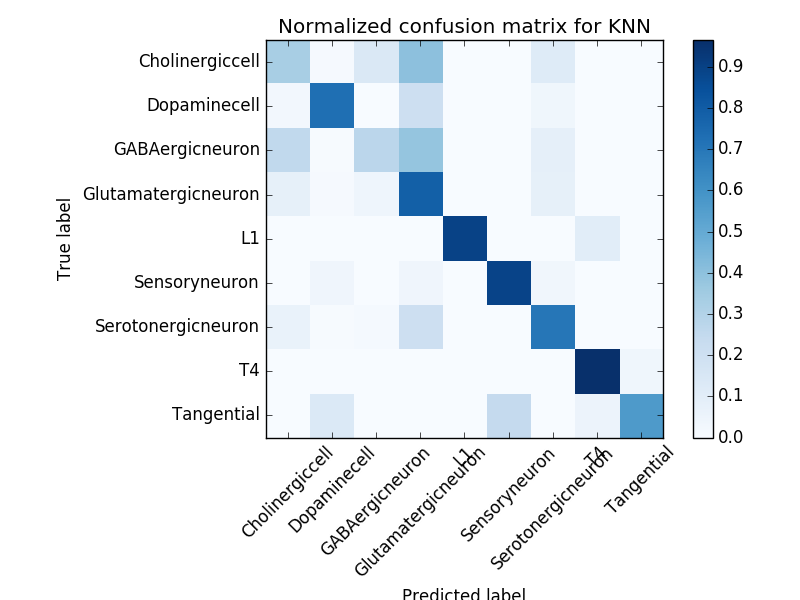
\includegraphics[width=\textwidth]{img/KNNmatrix.png}
		\caption{A Rectangle} 
		\label{fig:rectangle} 
	 \end{minipage}
\end{figure}

\begin{figure}[htbp] 
	\begin{minipage}{0.5\linewidth} 
		\centering 
		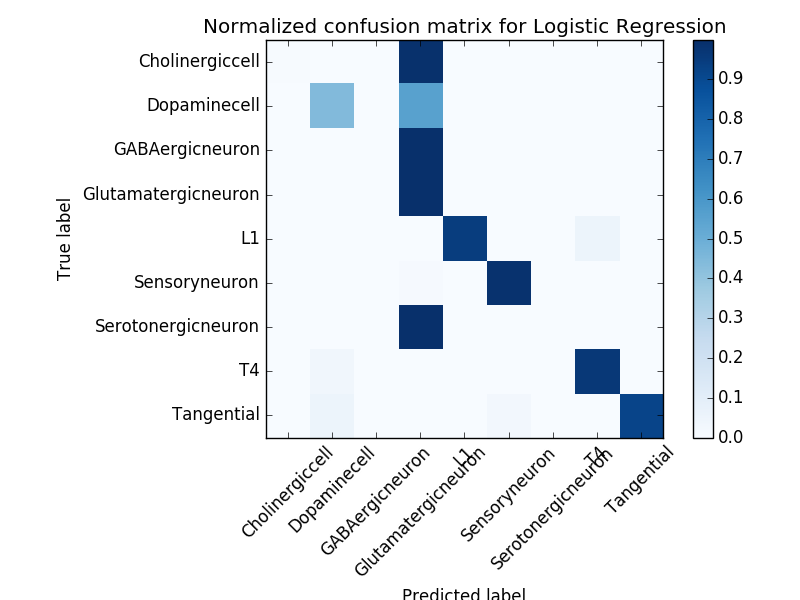
\includegraphics[width=\textwidth]{img/LGmatrix.png} 
		\caption{A Circle} 
		\label{fig:circle} 
	\end{minipage}% 
	\begin{minipage}{0.5\linewidth} 
		\centering 
		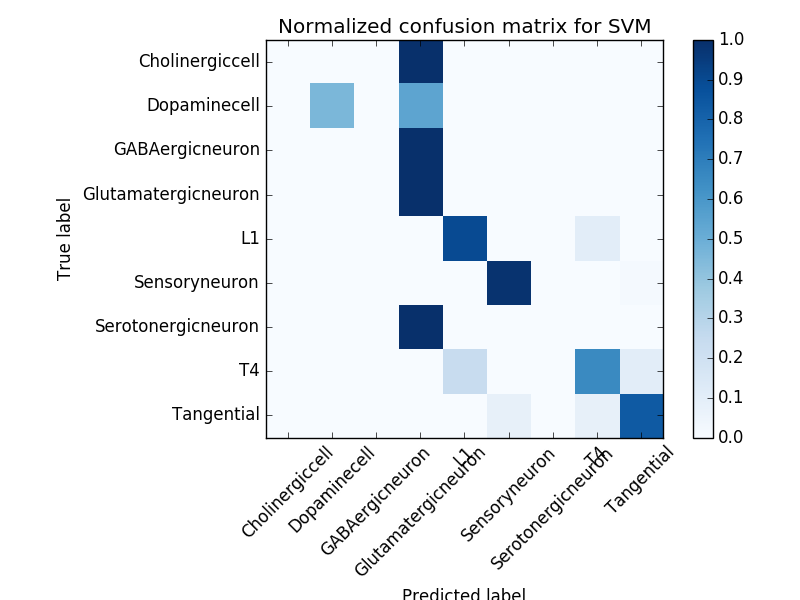
\includegraphics[width=\textwidth]{img/SVMmatrix.png}
		\caption{A Rectangle} 
		\label{fig:rectangle} 
	\end{minipage}
\end{figure}	

\begin{figure}[htbp] 
	\begin{minipage}{0.5\linewidth} 
		\centering 
		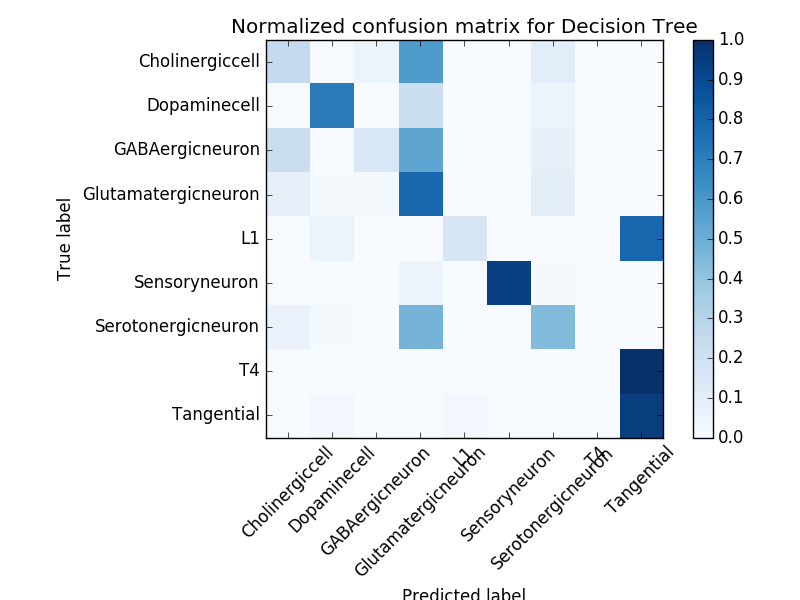
\includegraphics[width=\textwidth]{img/DTmatrix.png} 
		\caption{A Circle} 
		\label{fig:circle} 
	\end{minipage}% 
	\begin{minipage}{0.5\linewidth} 
		\centering 
		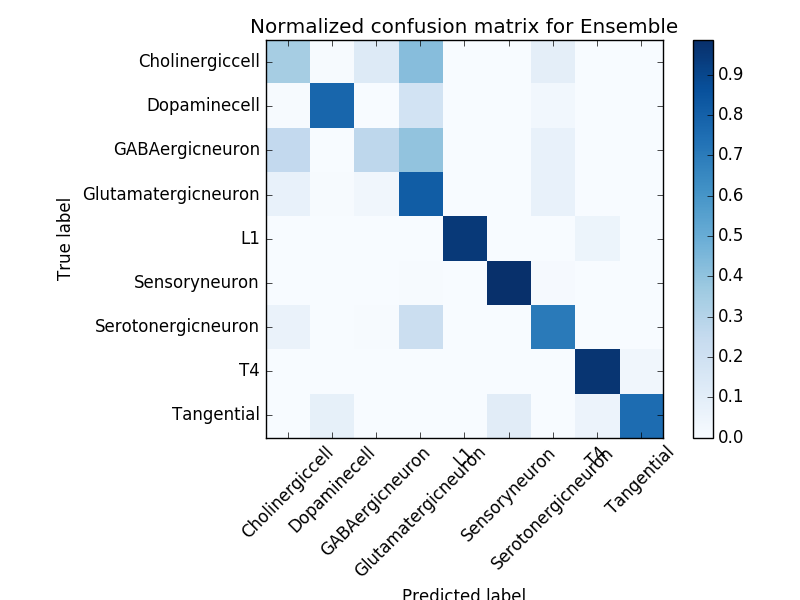
\includegraphics[width=\textwidth]{img/ENSEMBLEmatrix.png}
		\caption{A Rectangle} 
		\label{fig:rectangle} 
	\end{minipage}
\end{figure}	

\begin{figure}[!ht]
	\centering
	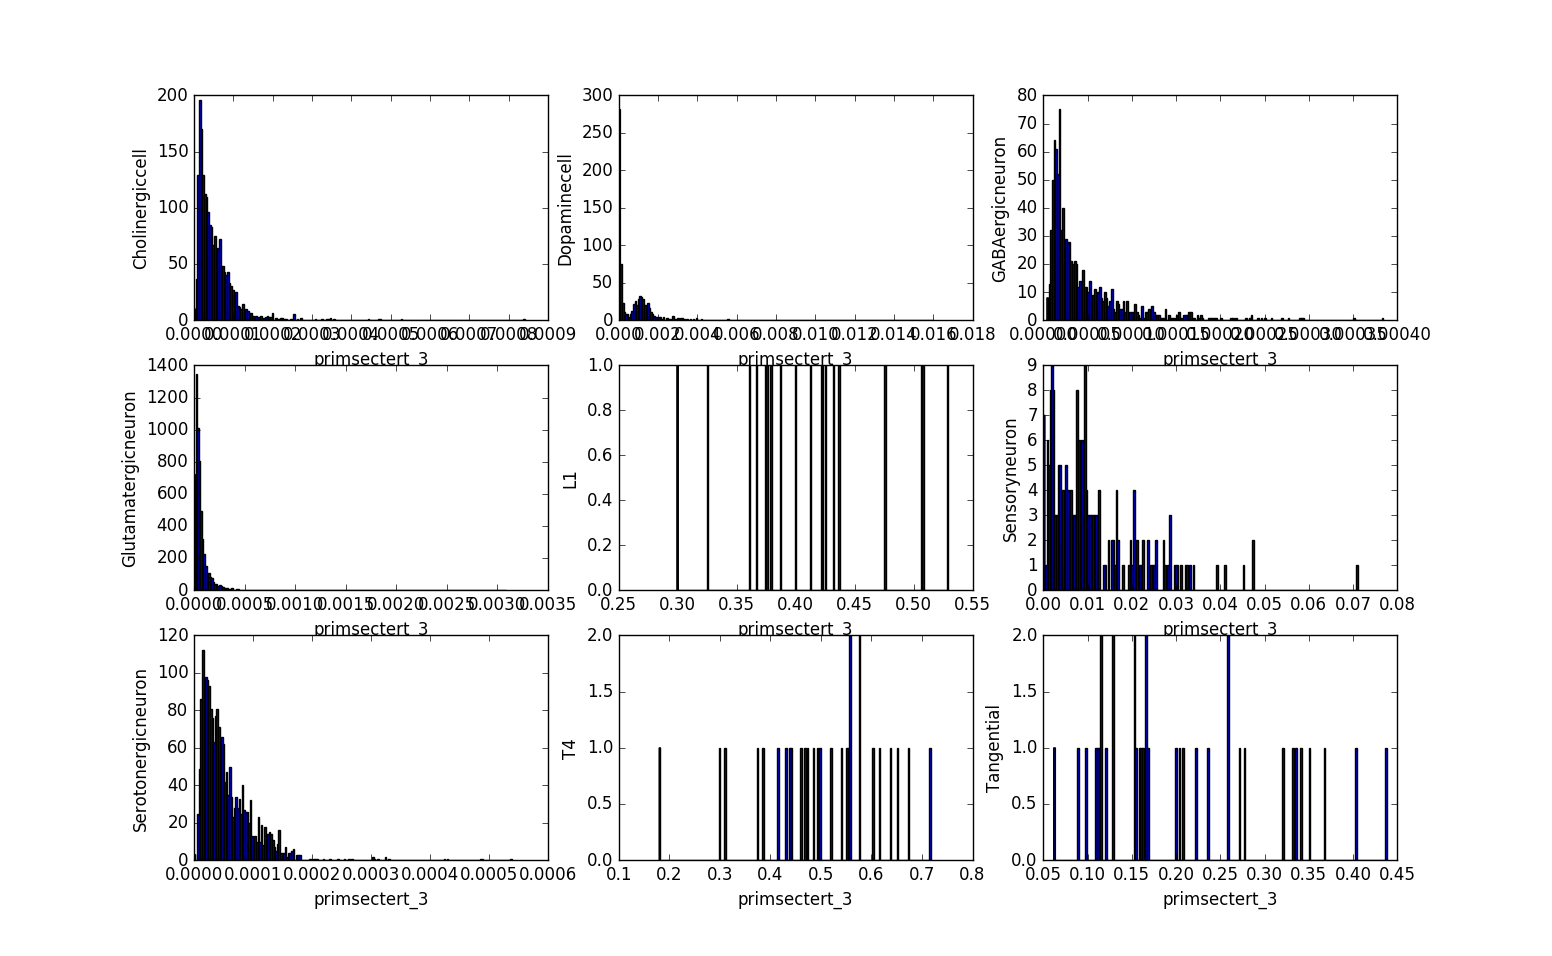
\includegraphics[width=0.5\textwidth]{img/test_fig.png}
	\caption{Figure something}
	\label{fig:chi2}
\end{figure}

\Section{Summary and Conclusions}

This template will get you through the minimum article, i.e., with no
figures or equations.  To include those, please refer to your LaTeX
manual and the IEEE publications guidelines.  However, for a vision
conference you will probably want the following equation somewhere:
$$g(x) = {1\over\sqrt{2\pi}\sigma}e^{-x^2/2\sigma^2}$$
Good Luck!

% This is how to do an unnumbered section (note asterisk).
\section*{Acknowledgments}

This is how to do an unnumbered subsection.  For submission, there
should be no acknowledgments as this could lead to identification
of the author.

\begin{thebibliography}{9}
\small  % Use 9 point text.

\bibitem{key:foo}
I. M. Author,
``Some Related Article I Wrote,''
{\em Some Fine Journal}, Vol. 17, pp. 1-100, 1987.

\bibitem{foo:baz}
A. N. Expert,
{\em A Book He Wrote,}
His Publisher, 1989.

\end{thebibliography}
\end{document}